% **************************************************
% Document Class Definition
% **************************************************
\documentclass[%
	paper=A4,	  				% paper size
	twoside,		   		    % oneside or twoside printing
	openright,					% doublepage cleaning ends up right side
	parskip=half,				% spacing value / method for paragraphs
	chapterprefix=true,			% prefix for chapter marks
	10pt,						% font size
	headings=normal,			% size of headings
	bibliography=totoc,			% include bib in toc
	listof=totoc,				% include listof entries in toc
	titlepage=off,				% 
	captions=tableabove,		% display table captions above the float env
	draft=false,				% value for draft version
]{scrreprt}%

% **************************************************
% Debug LaTeX Information
% **************************************************
%\listfiles

% **************************************************
% Information and Commands for Reuse
% **************************************************
\newcommand{\thesisTitle}{Improving the Measurement Accuracy of FSR Based Finger Force and Finger Position Measurements for String Instruments}
\newcommand{\thesisName}{Nico Haenni}
\newcommand{\thesisSubject}{Semester Thesis}
\newcommand{\thesisDate}{July 2018}

\newcommand{\thesisFirstSupervisor}{Tobias Grosshauser, ETZ H63}
\newcommand{\thesisSecondSupervisor}{Alberto Calatroni, ETZ H63}
\newcommand{\thesisUniversity}{\protect{ETH Z\"urich}}
\newcommand{\thesisUniversityDepartment}{Department of Information Technology and Electrical Engineering}
\newcommand{\thesisUniversityInstitute}{Institute for Integrated Circuits}


% **************************************************
% Load and Configure Packages
% **************************************************
\usepackage[utf8]{inputenc}		% defines file's character encoding
\usepackage[english]{babel} % babel system, adjust the language of the content
\usepackage[pdftex,dvipsnames]{xcolor}  %colored text etc...

\usepackage[colorinlistoftodos,prependcaption,textsize=tiny]{todonotes}  % package to add notes in text
%\usepackage[disable]{todonotes}  %uncomment to hide notes


\usepackage{xargs}                      % Use more than one optional parameter in a new commands

\newcommandx{\unsure}[2][1=]{\todo[linecolor=red,backgroundcolor=red!25,bordercolor=red,#1]{#2}}
\newcommandx{\change}[2][1=]{\todo[linecolor=blue,backgroundcolor=blue!25,bordercolor=blue,#1]{#2}}
\newcommandx{\info}[2][1=]{\todo[linecolor=OliveGreen,backgroundcolor=OliveGreen!25,bordercolor=OliveGreen,#1]{#2}}
\newcommandx{\improvement}[2][1=]{\todo[linecolor=Plum,backgroundcolor=Plum!25,bordercolor=Plum,#1]{#2}}

\newcommandx{\thiswillnotshow}[2][1=]{\todo[disable,#1]{#2}}


\usepackage[					% clean thesis style
	figuresep=colon,%
	sansserif=false,%
	hangfigurecaption=false,%
	hangsection=true,%
	hangsubsection=true,%
	colorize=full,%
	colortheme=bluegreen,%
	bibsys=biber,%
	bibfile=bib-refs.bib,%
	bibstyle=ieee,%
]{cleanthesis}
\addbibresource{bib-refs.bib}


\usepackage{xfrac} % slanted fractions

\usepackage{algorithm}
\usepackage{algpseudocode}

%\usepackage[norelsize, ruled]{algorithm2e} % Provides the algorithm environment
\usepackage{tabularx} % Provides stretchable tables.
%\usepackage{bm} % Provides bold greek math symbols.
\usepackage{pdfpages} % Allows to include pdf documents.
\usepackage{pdflscape} % Rotate PDF pages in output
\usepackage{booktabs} % Provides nicer tables than the standard tables.
%\usepackage[figuresleft]{rotating}
%\usepackage{capt-of}% Provides more customizeable captions.
%\usepackage{caption}
\usepackage{graphicx} % Graphic Inclusion
\graphicspath{ {images/} }  

\usepackage[binary-units=true, detect-all]{siunitx} % SI Units
\usepackage{subcaption} % Provides the <subfigure> environment for placing multiple figures side-by-side and add separate Captions.
\usepackage{mathtools}

\DeclarePairedDelimiter{\floor}{\lfloor}{\rfloor}

\DeclareSIUnit\CHF{CHF}

\usepackage{tikz}
\usetikzlibrary{positioning}

\usepackage{amsmath}
\usepackage{amsfonts}
\usepackage{hyperref}

\hypersetup{					% setup the hyperref-package options
	pdftitle={\thesisTitle},	% 	- title (PDF meta)
	pdfsubject={\thesisSubject},% 	- subject (PDF meta)
	pdfauthor={\thesisName},	% 	- author (PDF meta)
	plainpages=false,			% 	-
	colorlinks=false,			% 	- colorize links?
	pdfborder={0 0 0},			% 	-
	breaklinks=true,			% 	- allow line break inside links
	bookmarksnumbered=true,		%
	bookmarksopen=true			%
}

%%%% 

%% Multiple Columns (for lists, etc..)
\usepackage{multicol}

%% Sideways Figures in Appendix
\usepackage{rotating}

%% Code Listing in Appendix
\usepackage{listings}

\lstset{
 basicstyle=\fontsize{8}{9}\ttfamily,
 commentstyle=\color{blue},
 keywordstyle=\color{red},
 frame=single,
 breaklines=true,
 keepspaces=true,
 breakindent= 0pt,
 columns = fullflexible
}

%% Typographic Corrections
\usepackage{microtype}

%% Fine-Control over Table of Contents (reduce Spacing)
\usepackage{tocloft}
\setlength{\cftbeforechapskip}{.9ex}
\setlength{\cftbeforesecskip}{.6ex}
\setlength{\cftbeforetoctitleskip}{.4ex}
\setlength{\cftaftertoctitleskip}{3em}


%% sloppy microtype paragraph, slightly compresses words.
%% Use as {\microtypecontext{expansion=sloppy}% your text...}
\SetExpansion
 [ context = sloppy,
 stretch = 20,
 shrink = 45,
 step = 1 ]
 { encoding = {OT1,T1,TS1} }
 { }

% force float to exact location with [H] (used in appendix)
\usepackage{float}

% highlight source code
\usepackage[]{minted}
\usemintedstyle{friendly}
\setminted{autogobble,breaklines,fontsize=\small,frame=lines}
\setmintedinline{breaklines=false,fontsize=\normalsize,frame=none}
\def\cppcode#1{\mintinline{cpp}{#1}}

% Remove large vertical spacing in enumerations
\usepackage[inline]{enumitem}
\setlist{leftmargin=*} 
\setlist[1]{labelindent=\parindent} 
\setlist{itemsep=0.7ex, parsep=0pt} % no vertical list separation

% Nicely Typeset C++, SqueezeNet++
\def\cpp{C{}\texttt{++}\xspace}
\def\squeezenetpp{SqueezeNet{}\texttt{++}\xspace}
\def\caffe{Caffe\xspace}

% Shortcuts for w/h/ch_in/out -> \wout, \hout, \chin, ...
\def\hin{\ensuremath{h_\textrm{in}}\xspace}
\def\win{\ensuremath{w_\textrm{in}}\xspace}
\def\chin{\ensuremath{ch_\textrm{in}}\xspace}
\def\hout{\ensuremath{h_\textrm{out}}\xspace}
\def\wout{\ensuremath{w_\textrm{out}}\xspace}
\def\chout{\ensuremath{ch_\textrm{out}}\xspace}
\def\npe{\ensuremath{N_\textrm{PE}}\xspace}


% Shortcut for $\times$
\def\x{$\times$}

% Hypenation Hints
\hyphenation{Squeeze-Net Zynq-Net In-cep-tion}

% Appendix Package 
\usepackage[title,titletoc]{appendix}

%% References with automatic Keywords (fig, sec, chap, ...)
\usepackage{cleveref}
%% Define "appendix" for cleveref
\crefname{appsec}{appendix}{appendices}


%%%%%%%% ADD LIST OF FIGURES / TABLES TO TOC
\KOMAoptions{listof=totoc}


% *******************************************
% ** Enable Vertical Lines in algorithmicx **
% *******************************************
\makeatletter
% start with some helper code
% This is the vertical rule that is inserted
\newcommand*{\algrule}[1][\algorithmicindent]{%
  \makebox[#1][l]{%
    \hspace*{.3em}% <------------- This is where the rule starts from
    \vrule height .75\baselineskip depth .25\baselineskip
  }
  \hspace*{-.6em}
}

\newcount\ALG@printindent@tempcnta
\def\ALG@printindent{%
    \ifnum \theALG@nested>0% is there anything to print
    \ifx\ALG@text\ALG@x@notext% is this an end group without any text?
    % do nothing
    \addvspace{-3pt}
    \else
    \unskip
    % draw a rule for each indent level
    \ALG@printindent@tempcnta=1
    \loop
    \algrule[\csname ALG@ind@\the\ALG@printindent@tempcnta\endcsname]%
    \advance \ALG@printindent@tempcnta 1
    \ifnum \ALG@printindent@tempcnta<\numexpr\theALG@nested+1\relax
    \repeat
    \fi
    \fi
}
% the following line injects our new indent handling code in place of the default spacing
\patchcmd{\ALG@doentity}{\noindent\hskip\ALG@tlm}{\ALG@printindent}{}{\errmessage{failed to patch}}
\patchcmd{\ALG@doentity}{\item[]\nointerlineskip}{}{}{} % no spurious vertical space
% end vertical rule patch for algorithmicx
\makeatother

% *************************************************
% Make a Glossary
% *************************************************
\definecolor{bluegray}{rgb}{0.4, 0.6, 0.8} % color that matches the theme

\usepackage[acronyms,toc,style=super,nonumberlist,nopostdot,nogroupskip]{glossaries}
%\renewcommand{\glsgroupskip}{}  %undoes grouping of acronyms starting with the same letter
\renewcommand{\glsnamefont}[1]{\textcolor{bluegray}{\textbf{#1}}}

\makenoidxglossaries
\loadglsentries{glossary}




% **************************************************
% Document CONTENT
% **************************************************
\begin{document}

% --------------------------
% rename document parts
% --------------------------
\renewcaptionname{english}{\figurename}{Fig.}
\renewcaptionname{english}{\tablename}{Tab.}


% --------------------------
% Front matter
% --------------------------
\pagenumbering{roman}			% roman page numbing (invisible for empty page style)
\pagestyle{empty}				% no header or footers
%!TEX root = ../tdc_project.tex

% --------------------------------------> main title page
\begin{titlepage}
	\pdfbookmark[0]{Titlepage}{Titlepage}
	\tgherosfont

 	\begin{center}
		\begin{minipage}[b]{0.45\linewidth}
			\begin{center}
 				\vspace{0pt}	
 				
\includegraphics[width=0.8\linewidth]{images./eth_logo.pdf}
				\hspace{1cm}
			\end{center}
		\end{minipage}
		\hfill
		\begin{minipage}{0.45\textwidth}
			\begin{center}
			\vspace{-1cm}
			\hspace{1cm}
 				%\includegraphics[width=0.8\linewidth]{scs_logo}
 				\flushright{Electronics Laboratory}
 				\vspace{-0.4cm}
                \flushright{Spring Semester 2018}
			\end{center}
		\end{minipage}
		
		\vspace{0.1cm}
		\hspace*{0.15cm}\rule{0.985\textwidth}{0.4pt}
		\vspace{0.1cm}
				
		{Semester Thesis Report}
		
		\vfill

		%{\Huge\textbf{ZynqNet:\\[6pt] An FPGA-Accelerated Embedded\\[10pt] Convolutional Neural Network}}
		{\Huge\textbf{Investigation and Design of a High 
Performance Digitally-Assisted Time Domain Data Converter for 5G DPLL
}}

		
		\vfill
		
		{\Large Nico Hänni}\\
		{nhaenni@student.ethz.ch}
		
		\vfill
		
		\begin{tabular}{ll}
		 Supervisors: & Tobias Grosshauser \\
		& Alberto Calatroni \\
		 \rule{0pt}{3ex}Professor: & Prof.\ Gerhard Tröster \\
		\end{tabular}\\[2mm]
		
		\vfill

		{July 2018, ETH Zürich,}\\[2mm]
		{Department of Information Technology and Electrical Engineering} \\[2mm]


 \end{center}

\end{titlepage}		% INCLUDE: title page
\cleardoublepage

\pagestyle{plain}				% display just page numbers
\section*{Abstract}

Modern electronics allowed us to integrate computational capabilities into everyday objects. In a world with an immense growth in sensor demand and production they still have not yet widely found their way into commonly used utilization for musical instruments. This creates space for further investigation in useful devices. Furthermore, sensor data accuracy plays an important role. Precise data are crucial for reliability.

This thesis investigates force sensing resistors (FSR) with application for accurate finger position and force exertion measurement. Used for musical instruments they can be used for educational purposes in a sense of detecting finger and hand posture and reveal poor force utilization, that could lead to exhaustion and sluggish note interchanges. Another useful application for the FSR would be a digital music sheet generator, by converting position measurement into midi files. A proper working real time conversion would then create a whole new horizon for augmented instruments.

The thesis presents a FSR system setup for position and area detection with an average error of less than 1.5mm. Based on position an offline algorithm to detect frequency of a played note on a fret instrument is presented.		% INCLUDE: the abstract
\cleardoublepage

%
%\input{content/acknowledgement} % INCLUDE: acknowledgement (not yet)
%\cleardoublepage

%
\setcounter{tocdepth}{2}	 	% define depth of toc
\tableofcontents				% display table of contents

\cleardoublepage

\printnoidxglossary[type=\acronymtype]
\printnoidxglossary[type=math]

\cleardoublepage

%%% LIST OF FIGURES
%\addtocontents{lof}{\protect\addcontentsline{toc}{chapter}{\listfigurename}}
%\phantomsection
\listoffigures 

\cleardoublepage

%%% LIST OF TABLES
%\addtocontents{lot}{\protect\addcontentsline{toc}{chapter}{\listtablename}}
%\phantomsection
%\listoftables

%\cleardoublepage


% --------------------------
% Body matter
% --------------------------
\pagenumbering{arabic}			% arabic page numbering
\setcounter{page}{1}			% set page counter
\pagestyle{maincontentstyle} 	% fancy header and footer


%
\section*{Introduction}
Playing a musical instrument involves complex motor tasks requiring certain postures, forces and coordinated movements. 
To observe these, the state-of-the-art systems can provide quite accurate results, but they all need cumbersome infrastructure, which restricts their usage to lab settings.
In the field of musicians' motion analysis, several video and marker based systems (see Ng et al.~\cite{Ng3MD2009}, Baader et al.~\cite{BaaderKazennikov2005-CoB} and \cite{GoeblPalmerTFA2008}) and electromagnetic positioning systems (like Pholemus) have been used until now. 
Still underrepresented in performance science research are force measurements and sensor based analysis systems. 
To improve these methods and making them more commonly usable, this thesis is focusing on the measurement precision of force sensitive resistors and linear potentiometers for finger force and position measurements for stringed instruments. 
With this technology objective observations and enhanced technical and artistic playing possibilities will possible in any surroundings and circumstances. % by simpler use compared to existing systems. 
% This thesis will evaluate the possibilities provided by capacitive finger position sensing (on the piano key), FSR based finger pressure sensing and wearable, wireless inertial measurement units (IMUs) for motion and hand/finger posture capturing.
Optionally wireless data transmission e.g.~via MIDI will be developed to allow connectivity and sound generation on computers and mobile phones. 
% Using wearable systems would open up plenty of possibilities to provide feedback to the musicians beginning with research during performances up to  practicing in daily life.
% Furthermore, other fields like practicing Yoga, rehabilitation, dancing (cite own paper?), etc. would benefit from a motion capturing and analysis system which is completely wearable.
\section*{Tasks}

The tasks of this thesis can be divided into the following categories and subtasks:

\subsection* {State of the Art and Literature Research}

% \subsection* {Introduction}
Sensing techniques in music are used in several fields. 
A short overview about the applications and usage of these technologies is the first step including investigations of existing most common digital music interfaces like OSC and Midi. 
% Further more the use of IMUs for finger sensing in musical instrument or alike interfaces playing should also be investigated and their feasibility evaluated. 

\subsection* {Setup of the Sensor System}

The goal of this part is to build a system consisting of FSR based force and linear potentiometer based position sensing and data fitting routines. 
Off the shelf and if possible, self printed sensors will be tested ( https://shop.agic.cc/collections/products/products/prototype-ink-kit) . 
With these sensors, the following experiments will be done: 
% Specifically, we seek finger position and force sensing under consideration of finger inclination: 


\subsection* {Experiments and Tests}

\begin{itemize}
\item  Pressure: a fitting algorithm for FSR based force raw values to N (Newton) already exists. But the influence of the contact size on the force measurement is still missing. We can estimate the contact area with a two sided measurement with linear potentiometers or with capacitive measurements. At least one of the two methods will be evaluated. 

\item  Position Measurement 1: Also the position depends on the pressure. We will examine linear potentiometers and finger position sensing accuracy with different  finger pressing forces. The goal is to find a fitting for position estimation in sub mm (Millimeter) range to recognize e.g. which tone is played. 

\item  Position Measurement 2: For note recognition (which is related to a specific finger position) on a musical instrument also the frequency can be used as ground truth. Frequency estimation usually takes too much calculation time for use real-time feedback scenarios, but it can be used to train the sensor based position recognition.  

\item [Optional:] Improving the Midi/OSC out implementation, partly already available. 

\item [Optional:] Adjusting the position raw values by changing the finger pressure on purpose. 

\end{itemize}



\section*{Realization of the Semester Thesis}

\subsection*{Abstract}
\begin{itemize}
\item
   \emph{Verification of Progress:} A metric for evaluating the progress is the comparison of the current achievements and the defined milestones. It has to be documented, if unexpected problems cause changes in the time schedule.
  \item
% HH: add workplace
   \emph{Workspace:} A PC equipped workspace is available in room H64, ETZ. 
     \item
   \emph{Initial Presentation:} Prepare a short presentation of your project at the very beginning of the work (5 minutes). 
  \item
   \emph{Final Presentation:} Present your achieved results at the end of the semester in the institute's colloquium.
  \item
   \emph{Meeting:} Discuss your achieved results and current problems with your supervisor or co-supervisor in frequent meetings.
 \end{itemize}
 
 \subsection*{Release}
 \begin{itemize}
  \item
   \emph{Report:} Provide three signed copies of your thesis to your supervisor until \AbgabeDatum \. Insert the present document to the beginning of the thesis.
  \item
   \emph{Homepage:} The most important results will be published on the institute's internal homepage. Prepare a short summary, therefore. 
  \item 
   \emph{Cleanup:} Clean up your local data, copy the most important to your Unix-Account. Burn all relevant data onto a CD-ROM and attach it to the report.
 \end{itemize}

\section*{Additional Information}
 \begin{itemize}
  \item
   A guideline for Semester- and Diploma Thesis that are written at the Electronics Lab (IfE), ETH, can be found at: (\url{http://www2.ife.ee.ethz.ch/repository/sada/SADA_Anleitung.pdf}).
 \end{itemize}

\dateandsignature 

\vspace{4cm}

\pagebreak



\section*{Abstract}

Modern electronics allowed us to integrate computational capabilities into everyday objects. In a world with an immense growth in sensor demand and production they still have not yet widely found their way into commonly used utilization for musical instruments. This creates space for further investigation in useful devices. Furthermore, sensor data accuracy plays an important role. Precise data are crucial for reliability.

This thesis investigates force sensing resistors (FSR) with application for accurate finger position and force exertion measurement. Used for musical instruments they can be used for educational purposes in a sense of detecting finger and hand posture and reveal poor force utilization, that could lead to exhaustion and sluggish note interchanges. Another useful application for the FSR would be a digital music sheet generator, by converting position measurement into midi files. A proper working real time conversion would then create a whole new horizon for augmented instruments.

The thesis presents a FSR system setup for position and area detection with an average error of less than 1.5mm. Based on position an offline algorithm to detect frequency of a played note on a fret instrument is presented.
\chapter{Force Sensors Overview}
\label{ch:overview}


This chapter is concerned about the basic functionality of force sensing resistor. A review of the technology is presented and typical characteristics are discussed. At the end the it is justified why using a FSR is used in extent of this thesis

\section{Previous Research}

Several techniques for the assessment of hand function have been devised over the past 70 years. Early methods focused on measuring dexterity rather than hand strength.\cite{nikonovas2004application} Used force sensors directly applied to the finger for hand positioning and force measurements. \cite{grosshauser2013finger} Applied a linear potentiometer directly on top of a violin fret to measure finger position.

\section{Force Sensing Resistors}


\section{FSR Technology Overview}
FSRs are polymer thick films (PTF) devices which exhibit a decrease in resistance when an external force is applied. The main composition can be broken into three main parts. A conducting and a resistive area which are separated by an adhesive spacer positioned at the verge of the FSR fig.\ref{fig:fsrcomposition}. The thickness of a FSR varies with desired design variables such as sensitivity and flexibility. At rest, the two polymer films do not touch each other, resulting in a non conductive state or high impedance. Once a force is exerted and contact between the two layers is established, the FSR becomes essentially a resistor.\newline
In contrast to load cells, FSR are not transducers. Neither are they strain gauges which rely on a change in resistance of a deformed resistor.\cite{giovanelli2016force}

\begin{figure}[ht]
    \centering
    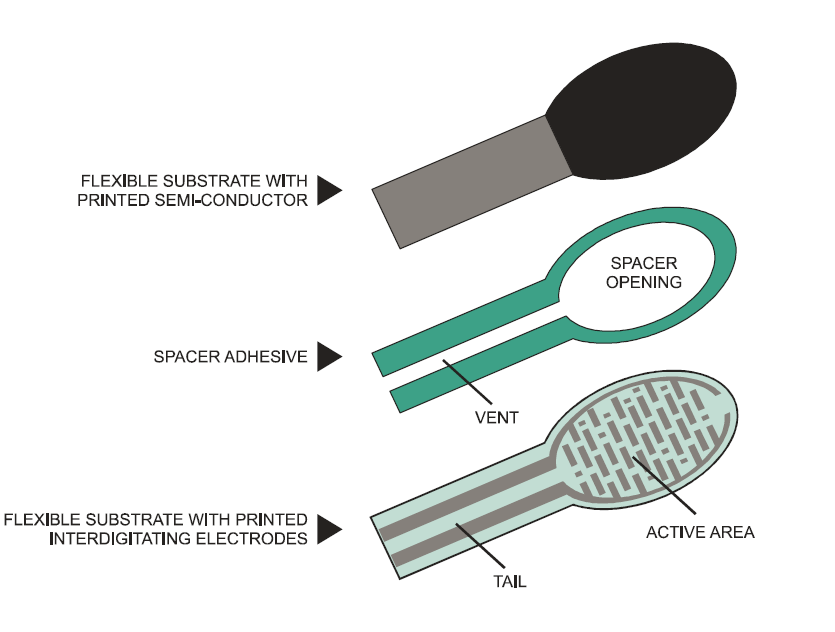
\includegraphics[width=0.75\textwidth]{images./fsr_parts.png}
    \caption[Individual Parts]{FSR individual parts. Source: \cite{interlinkelectronics}}
    \label{fig:fsrcomposition}
\end{figure}

\subsection{Sensor Setup}
\label{subsection:setup}
A typical senor setup is given in \ref{fig:setup}. The voltage drop across the load resistance is to be measured to lead back on the R\textsubscribt{F} value. In this configuration, the output voltage increases with increasing exerted force to the FSR as to be seen in fig \ref{fig:forcevalues}. If the resistors R\textsubscribt{FSR} and R\textsubscribt{L} were swapped, the output would decrease starting from supply voltage. The voltage across the load resistance can be described by a simple voltage divider:
\begin{equation}
    V_{out}=\frac{V_{dd}\cdot R_L}{R_L+R_{FSR}}
    \label{eq:divider}
\end{equation}
\begin{figure}[ht]
    \centering
    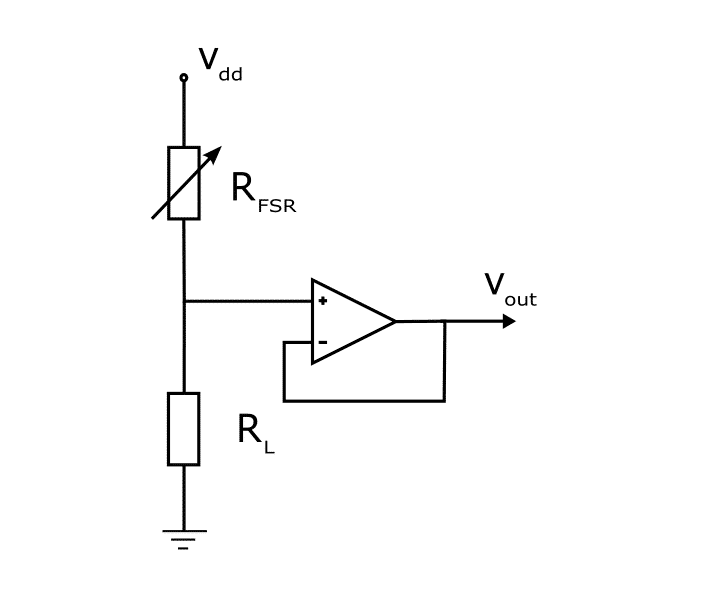
\includegraphics[width=0.75\textwidth]{images./FSR-1.png}
    \caption[FSR Setup]{Typical FSR Setup}
    \label{fig:setup}
\end{figure}




\section{FSR Performance Characteristics}
This section will be concerned about general characteristics of FSRs. Important to note at this point, that they are neither true force nor true pressure sensor, because of their area dependency on the measuring resistor. A true force sensor will always yield to the same signal for the same applied force regardless of position and area. 

\subsection{Force vs Resistance/ Conductance}
Fig \ref{fig:forcevalues} shows a typical characteristic of applied force versus measured voltage. For this characteristic, normed weights up to 1.6kg on a constant area of 3.5mm\textsuperscript{2} were used. It can bee seen that the force sensing resistor decreases in a non linear matter, at the high force end of the dynamic range, the response deviates from the power-law behavior, and eventually saturates to a point where increases in force yield little or no decrease in resistance. The saturation pressure of a typical FSR is in the order of 7 to 14 bar \cite{interlinkelectronics}.
\begin{figure}[ht]
    \centering
    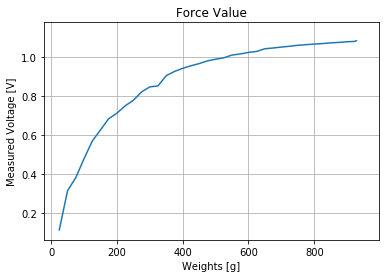
\includegraphics[width=0.75\textwidth]{images./Force.png}
    \caption[Force Characteristic]{Force Voltage Characteristic}
    \label{fig:forcevalues}
\end{figure}

\subsection{Accuracy}
\label{subsection:accuracy}
With proper mechanical arrangement, repeatability of an individual FSR is better than $\pm$ 2 \% over a specified force range. Variation between FSRs of a type is typically $\pm$ 15 \% \cite{yaniger1991force}. 




\section{Three Port Sensor}
In this thesis for the experiments a long FSR with an additional port on the resistor layer was used, see fig\ref{fig:scematic}. That additional port essentially turns the resistive layer into a linear potentiometer depending on force position.

which additionally allows position measurement. The schematic is presented in \ref{fig:FSR}.

\subsection{Sensor Schematic}
Figure \ref{fig:simplified} shows a simplified version of the given FSR. When pressure is applied on the surface the resistive layer at the bottom gets contact to the conductive layer hence creating a change in resistance. Resistor R\textsubscribt{F} is variable with contact size and force where R\textsubscribt{1} and R\textsubscribt{2} depend on position and area of the applied force. The corresponding schematic can be seen in fig. \ref{fig:schematic}



\begin{figure}[htp]
    \centering
    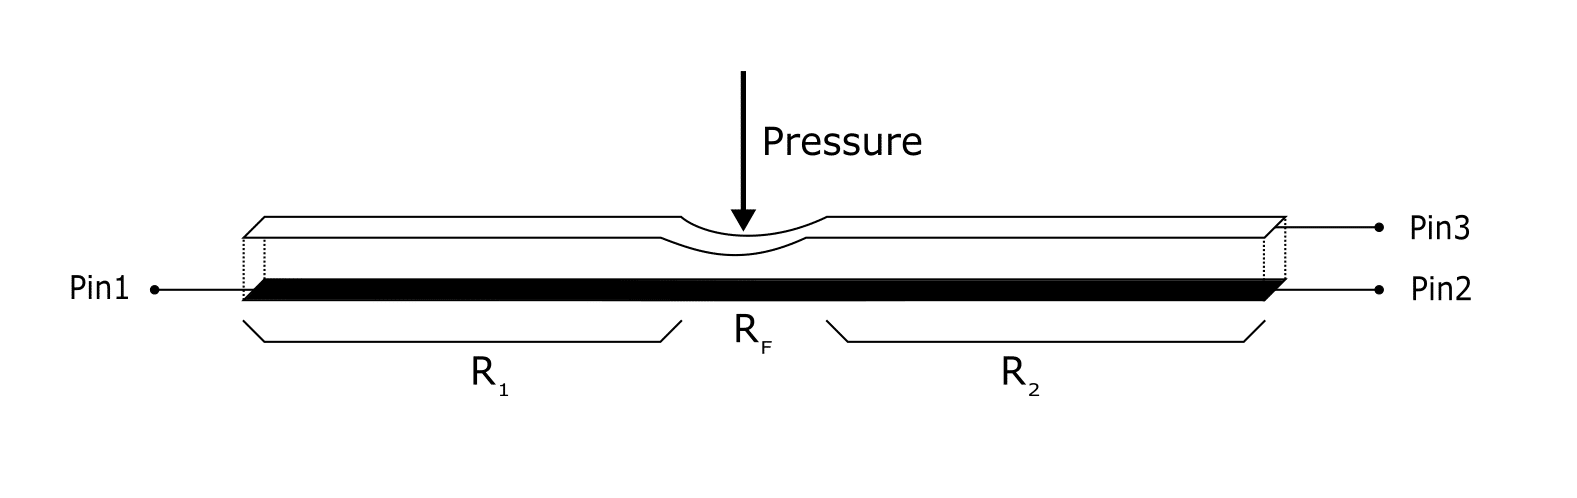
\includegraphics[width=\textwidth]{images./ForceSensor-1.png}
    \caption[FSR simplified]{Simplified Depcition}
    \label{fig:simplified}
\end{figure}  

\begin{figure}[htp]
    \centering
    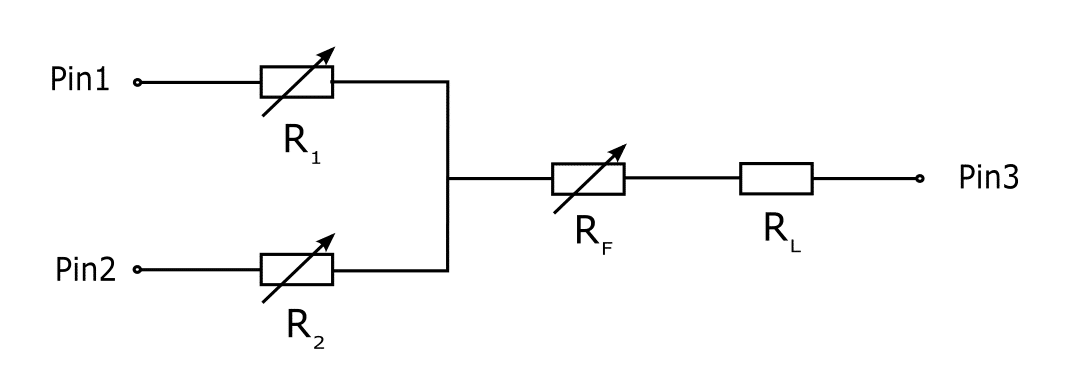
\includegraphics[width=\textwidth]{images./breakdown.png}
    \caption[FSR Schematic]{FSR Schematic}
    \label{fig:schematic}
\end{figure}  

\section{Operation Principle}

\chapter{Proposed System}

In this section the full sensor setup is described step by step and design choices are justified. In the first part the concept of different modes are presented.



\section{Operating Modes}

In order to measure the information carrying signals, respectively the resistor values as described in section \ref{sec:3port}, the voltage supply on the pins has to be switched. The resistor values can be then used to detect position. Mode 1 in fig. \ref{fig:operatingmode} shows the arrangement how the voltage drop over R\textsubscript{1} is measured by the voltage divider in equation \ref{eq:divider}. For the following equation the terminology R(F) is used, where "F" refers to force dependency. Therefore as mentioned already in chapter \ref{ch:overview} the FSR is no true force sensor due to the area dependency.\newline
An alternative solution to the system presented here would be to have load resistances at the pins connected to R\textsubscript{1} and R\textsubscript{2}. The only difference would be that e.g. in the first mode when no force is applied the signal would be zero instead of the supply voltage as it is in the presented arrangement. Then if force was applied signal would rise instead of drop. However, as already mentioned in \ref{subsection:setup} it would not make any difference for the measurements. For this method an additional resistor and an additional pin on the PSoC would have been needed and therefore the initial presented method was used.

\begin{figure}[htp]
    \centering
    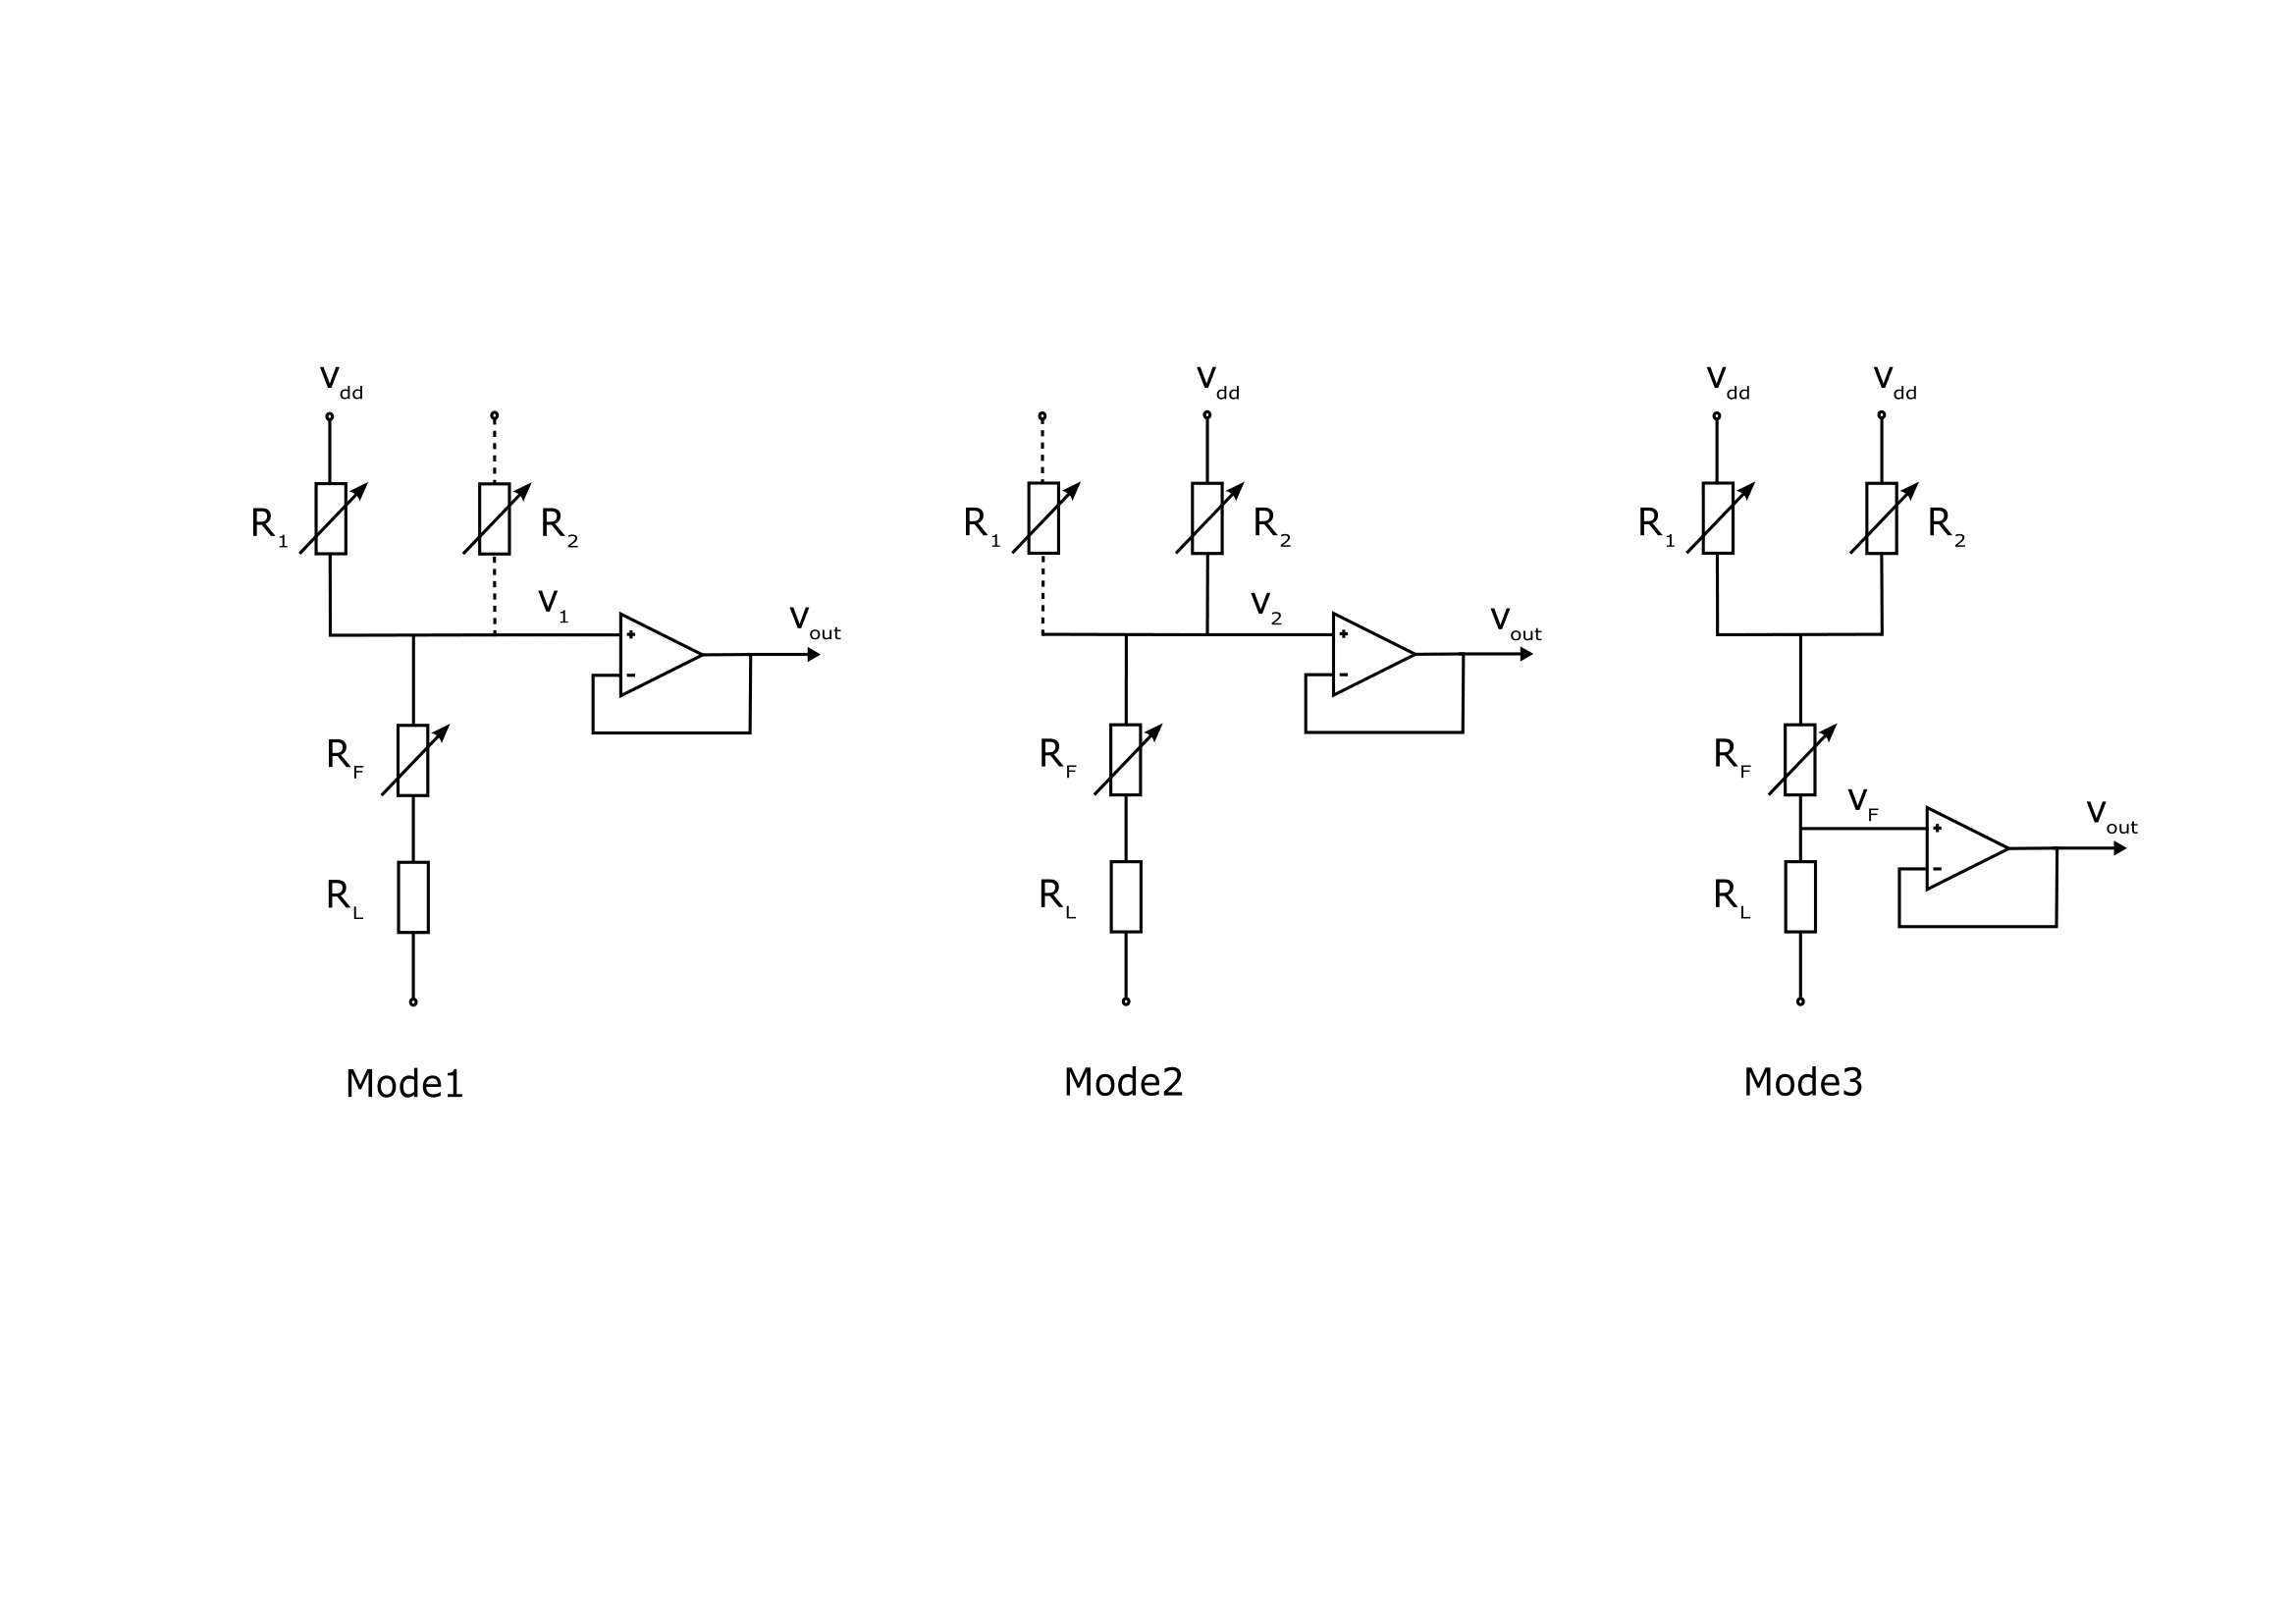
\includegraphics[width=\textwidth]{images./3MODES-1.png}
    \caption[Proposed system overview: System level]{3 operating modes}
    \label{fig:operatingmode}
\end{figure}  





\begin{equation}
    \frac{R_1(x)}{V_1(x)}=\frac{V_{dd}}{R_1(x)+R_r(F)+R_L}
    \label{eq:divider}
\end{equation}
leading to:
\begin{equation}
    R_1(x)=R_F(F)\cdot(\frac{V_{dd}}{V_1(x)}-1)
    \label{eq:r1}
\end{equation}
The same is valid for the second mode: 
\begin{equation}
    R_2(x)=R_F(F)\cdot(\frac{V_{dd}}{V_2(x)}-1)
    \label{eq:r2}
\end{equation}
For the third mode both Pin\textsubscript{1} and Pin\textsubscript{1} are set to logic high and the value of R\textsubscript{F} is measured. Also a voltage divider results in:
\begin{equation}
    \frac{V_F}{R_F(F)}=\frac{V_{DD}}{R_1(x)//R_2(x)+R_F(F)+R_L}
\end{equation}
\begin{equation}
    R_F(F)=\frac{R_1(x)\cdot R_2(x)}{(R_1(x)+R_2(x))}\cdot \frac{V_F}{V_{dd}-V_F}
    \label{eq:rf}
\end{equation}
Using equation \ref{eq:r1} and \ref{eq:r2}:
\begin{equation}
    R_F(F)=\frac{R_F^2(\frac{V_{dd}}{V_1}-1)(\frac{V_{dd}}{V_2}-1)}{R_F\cdot (\frac{V_{dd}}{V1}+\frac{V_{dd}}{V2}-2 )} \cdot \frac{V_F}{V_{dd}-V_F}
    \label{eq:underdtermined}
\end{equation}
Unfortunately \ref{eq:underdtermined} shows that the determinant of this system is zero, or in other words the system is non invertible. Therefore no unique solution for the system can be found. For the experiments in chapter \ref{ch:results} the load resistance is set a lot higher than the force depending resistor leading to accurate results even when ignoring the variation of R\textsubscript{F}.




\subsection{Switching modes}
Modern FSR have a typical rise time of no more than three microseconds  \cite{datasheet}. For a meaningful measurement each of the three modes has to be evaluated, resulting in force, area and position information. The microcontroller on a PSoC prototyping kit was programmed to transmit a sample and then switch to the next mode. Between each change of a mode there was a safety delay of 10ms introduced, still leading to a acceptable resolution while eliminating all possible rise time errors.




\subsection{Software}
\chapter{Results and Evaluation}
\label{ch:results}
The main in goal of this thesis was to analyze the relation between force, area and position of the presented FSR and create a data fitting routines to estimate contact size, exerted force and position. In this chapter the results of the thesis are presented and its accuracy evaluated.


\section{Measurements}



\subsection{Position}

One task of the thesis was to evaluate accuracy of the given FSR and identify whether it was possible to set up a sensor system detecting position within sub millimeter range.

\begin{figure}%
    \centering
    \subfloat[Raw]{{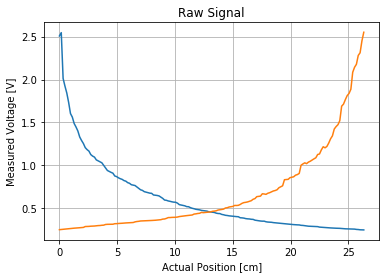
\includegraphics[width=5cm]{images./Positionraw.png}} }
    \label{fig:rawpos}
    \qquad
    \subfloat[Converted]{{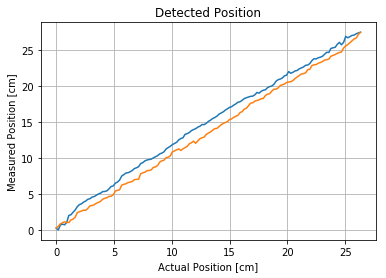
\includegraphics[width=5cm]{images./Position.png}} }
    \caption{2 Figures side by side}%
    \label{fig:positions}%
\end{figure}

\subsection{Area vs Force}

\begin{figure}[htp]
    \centering
    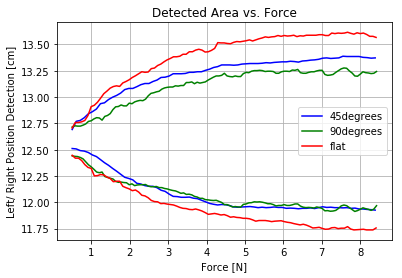
\includegraphics[width=10cm]{images./ForcevsArea.png}
    \caption[Area Detection]{Exerted Force }
    \label{fig:operatingmode}
\end{figure}  

\subsection{Accuracy}




As mentioned in \ref{subsection:accuracy} deviation \todo{graph with deviation}





\cleardoublepage


%%%%%%%%%% APPENDIX %%%%%%%%%%%%%%%%

\begin{appendices}
\let\cleardoublepage\clearpage % Begin Appendix Chapters on next Page (left or right)
\crefalias{section}{appsec} % Use cleveref "appendix A.1, appendix C, ..." for sections and chapters in appendix
\crefalias{chapter}{appsec}
\chapter{Code}

\section{PSoC Code}
\section{Python Code}

   %marked as comment as file not yet existent (Christian)

\end{appendices}


{%
\setstretch{1.1}
\renewcommand{\bibfont}{\normalfont\small}
\setlength{\biblabelsep}{0pt}
\setlength{\bibitemsep}{0.5\baselineskip plus 0.5\baselineskip}
\printbibliography[nottype=online]						
\printbibliography[heading=subbibliography,title={Websites},type=online] 

}


% --------------------------
% List of notes in Text
% --------------------------
%\newpage
%\listoftodos[Notes]

% **************************************************
% End of Document CONTENT
% **************************************************
\end{document}
